\begin{problem}
\quad 図1のように2つの正方形ABCDとCDEFを並べた図形を考える.\, 2点P,Qが6個の頂点A,B,C,D,E,Fを以下の規則(a),(b)に従って移動する.
\begin{enumerate}[(a)\ ]
  \item 時刻0では図2のように点Pは頂点Aに,点Qは頂点Cにいる.
  \item 点P,Qは時刻が1増えるごとに独立に,今いる頂点と辺で結ばれている頂点に等確率で移動する.
\end{enumerate}
\quad 時刻$n$まで2点P,Qが同時に同じ頂点にいることが一度もない確率を$p_n$と表す.\, また時刻$n$まで2点P,Qが同時に同じ頂点にいることが一度もなく,かつ時刻$n$に2点P,Qがともに同じ正方形上にいる確率を$a_n$と表し,$b_n=p_n-a_n$と定める.\, このとき,次の問に答えよ.\\
\begin{enumerate}
  \item 時刻1での点P,Qの可能な配置を,図2にならって全て図示せよ.
  \item $a_1,b_1,a_2,b_2$を求めよ.
  \item $a_{n+1},b_{n+1}をa_n,b_nで表せ.$
  \item $p_n \leq \left(\bunsuu{3}{4}\right)^nを示せ.$
\end{enumerate}
\begin{center}
\begin{tikzpicture}
  \draw(2,0)--(8,0)--(8,-3)--(2,-3)--cycle;
  \draw(5,0)--(5,-3);
  \draw(2,0)node[above]{A};
  \draw(5,0)node[above]{D};
  \draw(8,0)node[above]{E};
  \draw(8,-3)node[below]{F};
  \draw(5,-3)node[below]{C};
  \draw(2,-3)node[below]{B};
  \coordinate[label=below:【図1】](【図1】) at (5,-3.5);
\end{tikzpicture}\hspace{15mm} %
\begin{tikzpicture}
  \draw(2,0)--(8,0)--(8,-3)--(2,-3)--cycle;
  \draw(5,0)--(5,-3);
  \draw(2,0)node[above]{P};
  \draw(5,-3)node[below]{Q};
  \fill[black] (2,0) circle(0.06);
  \fill[black] (5,-3) circle(0.06);
  \coordinate[label=below:【図2】](【図2】) at (5,-3.5);
\end{tikzpicture}
\end{center}
\end{problem}


\kaie
\begin{enumerate}
  \item 時刻1における2点P,Qの可能な配置は,以下の6つの場合のみである.
  \item(1)の図より,$p_1=\bunsuu{1}{6}, a_1=\bunsuu{1}{2}, b_1=p_1-a_1=\bunsuu{1}{3}.$\\
  \qquad $a_2,b_2について考える.以下のように,事象X,Y,Zを定める.$
  \begin{align*}
    \left\{
    \begin{array}{ll}
     事象X:2点P,Qが正方形の対角線上にいる. \\
     事象Y:2点P,Qが(A,E),(B,F)のどちらかの組合せでいる.\\
     事象Z:2点P,Qが同じ頂点にある.
    \end{array}
    \right.
  \end{align*}
  \begin{enumerate}[(i)\ ]
    \item 時刻$kにおいて事象Xの場合$\\
    このとき,時刻$k+1で事象Xとなるのは\bunsuu{1}{2}, 事象Yとなるのは\bunsuu{1}{6}, 事象Zとなるのは\bunsuu{1}{3}の確率である.$
    \item $時刻kにおいて事象Yの場合$\\
    このとき,時刻$k+1で事象Yとなるのは\bunsuu{1}{2}, 事象Yとなるのは\bunsuu{1}{4}, 事象Zとなるのは\bunsuu{1}{4}の確率である.$
    \item $時刻kにおいて事象Zの場合$\\
    $時刻nから時刻n+1になるまでの推移に注目する.$
    \begin{center}
      \begin{tikzpicture}
      \draw(0,0)--(9,0);
      \coordinate[label=above:$時刻n$]($時刻n$) at (2,0);
      \coordinate[label=above:$時刻n+1$]($時刻n+1$) at (6,0);
      \coordinate[label=below:$X$]($X$) at (2,-0.2);
      \coordinate[label=below:$Y$]($Y$) at (2,-1.2);
      \coordinate[label=below:$X$]($X$) at (6,-0.2);
      \coordinate[label=below:$Y$]($Y$) at (6,-1.2);
      \draw[->] (3,-0.5)--(5,-0.5);
      \draw[->,thick] (3,-0.6)--(5,-1.4);
      \draw[->,thick] (3,-1.4)--(5,-0.6);
      \draw[->,dashed] (3,-1.5)--(5,-1.5);
      \end{tikzpicture} \hspace{15mm}%
      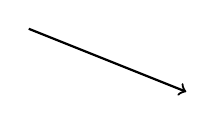
\begin{tikzpicture}
        \draw[->,thick] (3,-0.6)--(5,-1.4);
      \end{tikzpicture}
    \end{center}
  \end{enumerate}
\end{enumerate}
